
%%% Local Variables:
%%% mode: latex
%%% TeX-master: t
%%% End:

\chapter{数据挖掘系统更新}
在上节的数据更新的基础上,深圳市交通仿真系统(二期) 分析挖掘的交通
指标数据也需要重新进行运算,获得最新的各类交通指标。 因此,需要在深圳市
交通仿真系统(二期) 已建成的数据挖掘系统基础上, 按照设计的计算机流程对
交通指标进行重新运算, 并更新原有系统后台的数据库。

\section{数据挖掘系统结构}
深圳市交通仿真系统( 二期) 建成的数据挖掘系统是一个标准的计算机软件
系统, 按照严格的数据流处理架构将数据挖掘的整个流程分为:数据载入、 数据挖掘、数据
入库和数据汇总四个部分。 

\begin{para}
\item[数据载入] 将以文件形态存在的原始动态交通数据载入到后台关系数据库中
\item[数据挖掘] 根据业务需求和数据特点设计数据挖掘算法,对动态交通数据进行挖掘运算,生成专题指标 
\item[数据入库] 将指标计算结果持久化到数据库中,形成中间成果库
\item[数据汇总] 将数据挖掘指标进行统计汇总,并推送到查询子系统的后台数据库中
\end{para}

具体的系统结构图如图\ref{fig:chp03_数据挖掘系统结构}所示。

\begin{figure}[ht]
  \centering
  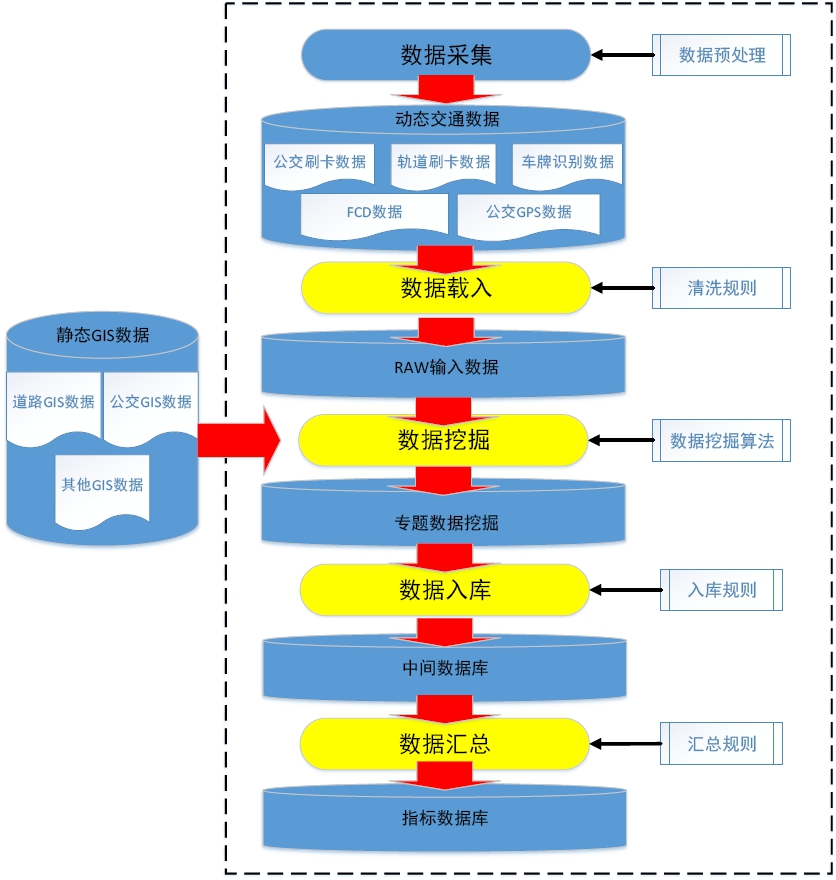
\includegraphics[width=0.85\textwidth]{chp03_数据挖掘系统结构.jpg}
  \caption{数据挖掘系统结构\label{fig:chp03_数据挖掘系统结构} }
\end{figure}

\section{更新后台数据库}
\subsection{数据载入}
在\charef{chp:数据更新}的数据更新工作中, 已经完成了原始数据的采集和预处理工作, 得到
了动态交通数据和静态 GIS 数据两个数据集。 数据载入的主要工作是将以文件
形态存在的原始动态交通数据转移(载入)到关系数据库中,为下一步处理步骤
(数据挖掘)做数据准备。在数据转移的过程中,会对数据进行基本的清洗过滤,
剔除那些格式不正确的数据。

由于动态数据预处理阶段只是对数据的格式进行标准化操作, 数据本身仍然
是原始数据,其中包含有数据传输过程中产生的错误、冗余和无效数据。 因此,
针对原始动态交通数据, 需要根据每种数据类型特点设定的清洗规则进行清洗,
获得可以用于数据挖掘计算的有效数据。

清洗后的有效数据存入数据挖掘后台数据库的数据表中,数据表全部以
RAW 开头,以下是所有清洗后数据表信息的说明。

\begin{longtabu} to \textwidth {|X|X[1,c]|X[0.85,c]|X|}
%\renewcommand\tabularxcolumn[1]{m{#1}}
\caption{清洗后的数据表结构\label{tbl:清洗后的数据表结构}}  
  \hline
  \multicolumn{1}{|c|}{\bfseries 表名} & \multicolumn{1}{c|}{\bfseries 表说明} &
  \multicolumn{1}{c|}{\bfseries 字段名} & \multicolumn{1}{c|}{\bfseries 字段说明}\\\hline
\multirow{4}*{RAW\_IC\_DATA} & \multirow{4}{=}{\centering 存储公交和轨道深圳通 IC 刷卡数据} & CARD\_ID & IC 卡 ID 编号\\\cline{3-4}
  & & TRADE\_DATE & 刷卡时间 \\\cline{3-4}
  & & TRADE\_TYPE & 交易类型 \\\cline{3-4}
  & & TERMINAL\_ID & 刷卡终端 ID 号 \\\hline
\multirow{4}*{RAW\_GPS\_DATA} & \multirow{4}*{存储公交GPS 数据} & LINE\_NAME & 公交线路 ID 编号\\\cline{3-4}
  & & BUS\_NAME & 公交线路名称 \\\cline{3-4}
  & & GPSTIME & GPS 时间戳 \\\cline{3-4}
  & & STATION & 公交到站站点 ID 号 \\\hline 
\multirow{4}*{RAW\_LP\_DATA } & \multirow{4}{=}{\centering 存储车牌识别数据} & PASS\_TIME & 识别时间戳  \\\cline{3-4}  
  & & DETECTOR\_ID & 识别点 ID 号 \\\cline{3-4}  
  & & CAR\_ID & 被识别车牌 \\\cline{3-4}  
  & & LANE & 车道\\
  \hline
\end{longtabu}

\subsection{数据挖掘}
数据挖掘主要功能是以数据载入生成的数据为输入, 根据交通规划的具体业
务需求和各类交通数据的特点设计专门的数据挖掘算法, 对动态交通数据进行全
方位的挖掘运算,生成各种专题挖掘数据,主要包括 15 分钟、 60 分钟和全天的
分时段指标数据。

数据挖掘的工作在深圳市交通仿真系统( 二期) 中已经开发了专门的数据挖
掘程序,可以进行全自动化作业。 数据挖掘的基本思路是:从表 10 中将数据库
后台的有效数据和相关静态 GIS 数据读取处理, 转换为 JAVA 对象并在内存中存
储, 然后按照数据挖掘的算法进行挖掘运算, 最后将运算结果按照一定的数据结
构存储在内存中,等待后续的数据入库操作。

虽然数据挖掘步骤实现了全自动化,但是在工作中也需要特别注意:

\smalltitle{更新 GIS 相关数据表}
数据挖掘系统后台数据库中有大量和 GIS 相关的数据表,表名以 GIS 开头。
由于前面已经进行了 GIS 数据图层的更新,因此在进行数据挖掘前要首先把 GIS
相关数据表也同步更新。

更新的方法是:首先删除后台数据库中原有 GIS 表的数据, 然后将\secref{sec:静态GIS数据处理}中
更新后的 shapefile 文件的属性数据导出为文本格式,最后再将文本格式文件导
入后台空的 GIS 表。

\smalltitle{防止重复处理}
输入数据表已经有被处理过的数据,例如,输入数据表中有 1 季度的数据,
并且已经处理过,现在载入 2 季度的数据进行处理, 就要指定数据挖掘的时间范
围, 可以在数据挖掘程序中通过设置 from 和 to 参数来实现。

\smalltitle{防止内存占用过高}
有些类型的数据在处理时,占用的内存资源会随着被处理数据数量的增加而
递增,例如出租车数据。为了避免一次处理太多的数据而导致处理程序内存溢出,
需要对数据进行分片多次处理。 根据之前的更新经验, 一次处理的数据不要超过
每种数据类型各一周。

\smalltitle{并行处理}
在系统资源允许的情况下,可以将原始数据按天为单位划分为多个任务进行
并行处理,可以大大加快数据的处理速度。

\smalltitle{错误异常处理}
如果在程序执行过程中发生异常,程序中断,导致只有部分数据被处理,结
果数据不完整,这时候需要重新执行任务。在重新执行任务时,必须将上一次处
理生成的部分结果数据删除, 否则在后续的数据入库流程中会产生数据库数据冗
余错误。

\subsection{数据入库}
上面的数据挖掘步骤将挖掘运算后的结果存储在内存中, 本节的数据入库工
作就是将内存中的计算结果, 插入到中间数据库中预先设计的数据表中。 这部分
工作全部由程序自动化完成。

针对每种数据类型和数据挖掘对数据的依赖关系,具体的数据入库工作分解
为 IC 刷卡数据、轨道数据、公交数据三个专题。 每类
数据的入库流程如下所示, 如果在数据入库中发生异常错误情况,可以根据入库
流程回溯到错误的初始位置。

\renewcommand{\arraystretch}{0.8}
\begin{longtable}[c] {|p{0.1\textwidth}|p{0.22\textwidth}|>{\baselineskip=14pt}m{0.2\textwidth}|m{0.36\textwidth}|} 
  \caption{数据挖掘成果入库表\label{tbl:数据挖掘成果入库表}}
  \hline
  \multicolumn{1}{|c|}{\bfseries 专题} & \multicolumn{1}{c|}{\bfseries 读取表} & 
  \multicolumn{1}{c|}{\bfseries 挖掘指标} & \multicolumn{1}{c|}{\bfseries 入库表}\\\hline
  \multirow[c]{5}*{刷卡数据} & \multirow[c]{5}*{RAW\_IC\_DATA} & \multirow[c]{3}*{分析换乘} & metro\_m2b\_line\_* \\
  & & & metro\_m2b\_station\_* \\
  & & & bus\_b2m\_line \\ \cline{3-4}
  & & \multirow[c]{2}*{分析刷卡概况} & metro\_ic\_overview \\
  & & & bus\_ic\_overview \\\hline
  
  \multirow[t]{16}*{轨道数据} & \multirow[t]{16}*{RAW\_IC\_DATA} & 线路流量 & metro\_line\_flow\_* \\*   %\\*表示行不允许跨页
  & & 站点流量 & metro\_station\_flow\_* \\\cline{3-4}
  & & 断面流量 & metro\_segment\_flow\_* \\\cline{3-4} 
  & & 小区流量 & metro\_zone\_flow\_* \\\cline{3-4}
  & & 吸引点流量 & metro\_sap\_flow\_* \\\cline{3-4}
  & & 站点 OD & metro\_od\_flow\_* \\\cline{3-4}
  & & \multirow{2}*{换乘} & metro\_transfer\_line\_flow\_* \\
  & & & metro\_transfer\_station\_flow\_* \\\hline
  & & 出行 OD & metro\_od\_zone\_flow\_* \\\cline{3-4}
  & & \multirow{2}*{平均距离} & metro\_dst\_man \\
  & & & metro\_net\_dst\_mean \\ \cline{3-4}
  & & \multirow{3}*{距离分布} & metro\_dst\_distance \\
  & & & metro\_dst\_station \\
  & & & metro\_dst\_elapse \\ \cline{3-4} 
  & & 吸引点 OD & metro\_sap\_od\_* \\\cline{3-4}
  & & 吸引点出行时长分布 & metro\_sap\_dst\_elapse \\\hline

  \multirow[c]{8}*{公交数据} & \multirow[c]{8}{=}{RAW\_GPS\_DATA RAW\_IC\_DATA} & 发车频率 & bus\_frequency\_60\\ \cline{3-4}
  & & 公交线段车速 & bus\_link\_speed\_60 \\\cline{3-4}
  & & 公交出行行程时间 & bus\_zone\_time\_* \\\cline{3-4}
  & & 站点流量 & bus\_station\_flow\_* \\\cline{3-4}
  & & 小区流量 & bus\_zone\_flow\_* \\\cline{3-4}
  & & 吸引点流量 & bus\_sap\_flow\_* \\\cline{3-4}
  & & 小区 OD 流量 & bus\_od\_zone\_flow\_*\\\cline{3-4}
  & & 站点 OD 流量 & bus\_od\_flow\_* \\\hline
 \end{longtable}

\subsection{数据汇总}
数据入库工作完成后,数据挖掘系统的工作已经全部完成, 但是考虑到在深
圳市交通仿真系统( 二期) 中,数据挖掘系统是数据查询系统的一个前置系统,
数据挖掘的数据需要通过数据查询系统来展现,因此数据挖掘后台的中间数据库
需要进一步统计汇总, 主要将中间数据库中的指标成果进行时段上的集聚, 形成
日间、夜间、 全天、 高峰时段等特征时段指标,再将汇总统计后的结果推送至数
据查询系统后台的指标数据库中。

由于在深圳市交通仿真系统( 二期) 已建成的系统中, 已经建立了数据挖掘
系统后台中间数据库与数据查询系统后台指标数据库相关表的对应关系,因此数
据汇总工作可以由程序自动化完成。 数据汇总后, 数据查询系统指标数据库中的
主要指标\tref{tbl:数据汇总后的交通指标}所示。\vfill

\begin{table}[!htpb]\centering
\renewcommand{\arraystretch}{1.2}
  \caption{数据汇总后的交通指标{\label{tbl:数据汇总后的交通指标}}} 
  \begin{tabular}{|m{0.12\textwidth}|m{0.48\textwidth}|m{0.25\textwidth}|}
    \hline
    \multicolumn{1}{|c|}{\textbf{数据类型}} & \multicolumn{1}{c|}{\textbf{基本指标}} &
    \multicolumn{1}{c|}{\textbf{时段}} \\ \hline
    轨道交通 & 线路客流、站点客流、轨道断面客流、站点 OD、换乘、出行距离/时间 & \multirow{3}{0.25\textwidth}{日间、夜间、全天、高峰时段}\\\cline{1-2}
    公交 & 总客流、线路客流、换乘 & \\\cline{1-2}
    道路交通 & 车牌识别点流量、车牌识别点间行程时间 & \\
    \hline
  \end{tabular}
\end{table}

\section{批处理更新操作}
由于数据挖掘系统输入数据的数据量大,而且数据挖掘各个流程中涉及的步
骤多且结构清晰, 因此很适合采用批处理模式针对每种挖掘流程进行自动化运算。

在批处理运行模式下,系统可以将数据载入、 数据挖掘、数据汇总等多个处
理任务,在批处理任务配置文件中定义,然后将该批处理任务提交给数据挖掘系
统,系统将自动执行这些任务,并将执行结果返回并入库。

\subsection{定义批处理配置文件}
批处理配置文件是自定义脚本文件,每行定义一个任务,所有任务都包含三个字段:

\begin{scriptcode}
GID;ID;TASK TYPE
\end{scriptcode}

\begin{para}
\item[GID] 任务组 ID,由数字组成,使用过的任务组 ID 不能再次使用;具有相
同 GID 的任务可以并行执行,具有不同 GID 的任务按照定义的先后顺序串行执
行
\item[ID] 任务 ID,由数字组成;表示该任务是任务组内的第几项任务;在同一
任务组内,任务 ID 不能重复
\item[TASK TYPE] 任务类型,代表不同的任务类型
\begin{cit}
\item \qd{x 或 X}:表示是否继续处理标志;如果任务组的最后一个任务的任务类型被
设置为 x,表示如果任务组内有任务执行失败,则中断整个批处理的执行
\item \qd{v 或 V}:表示定义变量任务; 通常放置在整个批处理配置文件首部,定义多
个后续任务可以引用的变量; GID 和 ID 通常都为 0
\item \qd{a 或 A}:表示数据载入任务;需要指定数据源参数
\item \qd{b 或 B}:表示数据挖掘任务;需要指定被分析数据的起始和截止日期
\item \qd{c 或 C}:表示数据汇总任务;需要指定汇总的年度参数
\item \qd{d 或 D}:表示数据库操作任务
\end{cit}
\end{para}

\smalltitle{V任务类型}
对于 V 类型的变量设置任务,包含以下变量设置字段:
\begin{scriptcode}
GID;ID;[v|V];VARIABLE DEF
\end{scriptcode}

其中,VARIABLE DEF变量设置任务是一个键值对,格式为“var=value”,等号前后不能有空格,
后续任务以“\${var}”方式引用该变量。例如:

\begin{examplecode}
0;0;v;year=2017
0;0;v;quarter=s3
0;0;v;day1=${year}0902
0;0;v;day2=${year}0903
...
11;1;a;ic;load.bus;/home/dm/data/${year}/${quarter}/ic/ic_bus_09.csv
11;0;x
...
21;1;b;ic;mine;${day1};${day2}
...
\end{examplecode}

对于 A、B、C 和 D 类型的任务,都包含以下两个字段:
\begin{scriptcode}
GID;ID;[a|b|c|d|A|B|C|D];TASK;PHASE
\end{scriptcode}

\begin{para}
\item [TASK] 任务分类
\begin{cit}
\item \qd{ic}:表示 IC 刷卡数据挖掘任务
\item \qd{metro}:表示轨道数据挖掘任务
\item \qd{bus}:表示巴士数据挖掘任务
\item \qd{road}:表示道路数据挖掘任务
\item \qd{taxi}:表示出租车数据挖掘任务
\item \qd{db}:表示数据库操作任务(只能用于 d 或 D 任务类型)
\end{cit}
\item [PHASE] 任务名称,为具体数据挖掘算法的执行步骤
\end{para}

\smalltitle{A任务类型}
对于 A 类型的数据载入任务,包含定义数据源的字段:
\begin{scriptcode}
GID;ID;[a|A];TASK;PHASE;DATA SOURCE
\end{scriptcode}
\begin{para}
\item[DATA SOURCE] 表示要载入的源数据;如果是文件,则指定文件的全路径名;
如果是关系数据库表,则通过“table:表名”格式指定
\end{para}

例如:
\begin{examplecode}
11;1;a;ic;load.bus;/home/dm/data/2017/s1/ic/ic_bus_09.csv
\end{examplecode}
\noindent{将生成: -task ic -phase load.bus -ds /home/dm/data/2014/s1/ic/ic\_bus\_09.csv 为
执行参数的任务。}

\smalltitle{B任务类型}
对于 B 类型的数据分析任务,包含定义被分析数据起止日期的字段:
\begin{scriptcode}
GID;ID;[b|B];TASK;PHASE;FROM;TO
\end{scriptcode}
\begin{para}
\item[FROM] 表示大于等于该日期的源数据,格式为“yyyyMMdd” 
\item[TO] 表示小于等于该日期的源数据,格式为“yyyyMMdd”
\end{para}

例如:
\begin{examplecode}
21;1;b;ic;mine;20170107;20170107
\end{examplecode}
\noindent{将生成:-task ic -phase mine -from 20170107 -to 20170107 为执行参数的任务。}

\smalltitle{C任务类型}
对于 C 类型的数据汇总任务,包含定义数据汇总年度的字段:
\begin{scriptcode}
GID;ID;[c|C];TASK;PHASE;ANNUAL
\end{scriptcode}
\begin{para}
\item[ANNUAL] 表示汇总数据的年度,格式为“yyyy”
\end{para}

例如:
\begin{examplecode}
31;1;c;ic;summary;2017
\end{examplecode}
\noindent{将生成: -task ic -phase summary -annual 2017 为执行参数的任务;}

\smalltitle{D任务类型}
在将数据载入时,通常都执行以下几个步骤:
\begin{nbeae}
\item 将目标表中的数据进行备份
\item 将目标表中的数据删除
\item 将目标表的索引失效(加快数据载入的速度)
\item 载入数据到目标表
\item 重建目标表的索引(加快后续的数据分析速度)
\end{nbeae}

因此,定义了 D 类型的数据库操作任务来完成上述过程:
\begin{scriptcode}
GID;ID;[d|D];TASK;PHASE
\end{scriptcode}
\begin{para}
\item[TASK] 字段固定为db
\item[PHASE] 字段支持以下几类操作:
\begin{cit}
\item \qd{backup.*}:将*中数据备份到*\_HIS 表中
\item \qd{truncate.*}:将*中数据删除
\item \qd{unusable.*.index}:使*的索引失效
\item \qd{rebuild.*.index}:重建*的索引
\end{cit}
\end{para}

例如:
\begin{examplecode}
# 将 raw_ic_data 表数据备份到 raw_ic_data_his 表
1;0;d;db;backup.ic
1;0;x

# 删除 raw_ic_data 表中的数据
2;0;d;db;truncate.ic
2;0;x

# 使 raw_ic_data 表的索引失效
3;0;d;db;unusable.ic.index
3;0;x

# 将数据载入到 raw_ic_data 表中
4;1;a;ic;load.bus;/home/dm/data/2013/s1/ic/ic_bus_09.csv
4;0;x

# 重建 raw_ic_data 表的索引
5;0;d;db;rebuild.ic.index
5;0;x
...
\end{examplecode}

\subsection{执行批处理任务}
执行批处理任务的命令如下:
\begin{scriptcode} master.sh [options] run|status \end{scriptcode}

\begin{para}
\item[run] 表示执行批处理任务
\item[status] 查看当前批处理任务运行状态
\item[options] 命令参数,其说明如下:
\begin{cit}
\item \qd{-f} 设定上节所定义的批处理任务文件
\item \qd{-r} 是否重新执行已完成的任务
\item \qd{-n} 表示查看任务运行状态界面的刷新间隔时间(秒),仅当执行status命令时生效
\end{cit}
\end{para}

当执行status命令查看任务运行状态时,包括以下几种情况:
\begin{para}
\item[Waiting] 表示任务处于等待执行状态
\item[Running] 表示任务正在执行 
\item[Completed] 表示任务已经成功完成
\item[Failed] 表示任务执行过程中发生异常
\item[Stopped] 表示任务对应的进程被终止 
\end{para}

通过查看运行状态,可以检查程序运行的健康程度。如果运行过程中出现问题,可以及时发现并排查问题。
\begin{nbeae}
\item 所有这些状态中,只有在“Running”状态下,有对应的操作系统进程存在;
\item 如果任务处于“Failed”状态,并且任务所属任务组设置了 x 中断标志,则整
个批处理任务将立即退出。这时,应该查看失败任务的日志,找到原因,排查处理,再重启任务(系统将跳过已完成的任务,重新执行失败的任务。如
果要重新执行已完成的任务,指定-r 选项;
\item 如果任务处于“Stopped”状态,是由于系统原因任务进程异常退出,通常任务还没有进入正式执行阶段(查看日志,确保没有进入正式执行)。这时,任务
会自动重启;如果连续 3 次自动重启都失败,批处理任务将退出。
\end{nbeae}

批处理任务一般以周为单位进行处理。每个季度有三周(每月一周)的数据,
因此通常会生成三个批处理任务定义文件。例如:对于第二季度的车牌识别数据,会生成三个批处理配置文件:lp4.cfg,
lp5.cfg, lp6.cfg,分别代表 4、5、6 月份的数据。要完成第二季度车牌识别数据挖
掘,就需要执行三个批处理任务:
\begin{examplecode}
$ bin/master.sh -f fcd4.cfg run
... 等待批处理完成
$ bin/master.sh -f fcd5.cfg run
... 等待批处理完成
$ bin/master.sh -f fcd6.cfg run
... 等待批处理完成
\end{examplecode}

需要特别注意的是,为了保证数据的一致性,执行批处理任务需要遵循下列原则:
\begin{nbeae}
\item 相同类型数据的多个批处理任务,只能串行执行,不能并行执行;
\item 不同类型数据的多个批处理任务,可以根据系统资源的实际情况并行处理。
\end{nbeae}

\subsection{批处理任务异常处理}
批处理过程中可以会因为内存不足、数据库存储空间不足、冗余数据插入、
载入数据未完全标准化等错误导致运行失败,出现异常情况。针对这些错误,数
据挖掘系统中有详细的日志文档,在系统运行的过程中会实时生成,当发生异常
时,需要人工去查看相应数据挖掘系统日志文档,根据对应的错误提示去解
决异常问题。

同时,在数据挖掘运算的过程中,数据挖掘系统提供了status命令去实时查看系
统运行的状态。常用的状态查看命令如下:

\smalltitle{查看当前批处理状态}
\begin{examplecode}
$ bin/master.sh -f lp4.cfg status
\end{examplecode}

\smalltitle{持续查看批处理状态,不断刷新(每 10 秒刷新一次)}
\begin{examplecode}
$ bin/master.sh -f lp4.cfg -n 10 status
\end{examplecode}
\noindent{在刷新状态下,会显示处于“Running”状态任务的最近一条日志信息。}

\smalltitle{查看任务日志}
批处理定义的每个任务都有单独的日志文件,存放在 log 目录下面,日志文
件名遵循下面格式:批处理文件名\_任务组ID\_任务ID.log。

\section{年度更新成果}
数据挖掘系统的年度更新成果包括:中间成果数据库和数据查询系统后台指
标数据库中的相关数据表,即在深圳市交通仿真系统(二期)已有数据的基础上
插入 \pyear 年的挖掘结果。其中中间成果数据库数据表共计 59 张,指标数据库数
据表共计 63 张,具体更新成果列表如下:

\renewcommand{\arraystretch}{0.8}
\begin{longtable}[c] {|C{0.22\textwidth}|>{\baselineskip=14pt}m{0.6\textwidth}|C{0.05\textwidth}|} 
  \caption{中间成果数据库更新表\label{tbl:中间成果数据库更新表}}
  \hline
  \multicolumn{1}{|c|}{\bfseries 类型} & \multicolumn{1}{c|}{\bfseries 表名} & 
  \multicolumn{1}{c|}{\bfseries 数量} \\\hline
GIS 相关 &公交线路、公交站点、道路网络、道路节点、道路检测点 & 5 \\\hline
IC 刷卡挖掘 & 轨道线路换乘公交客流量(60 分钟、全天)、轨道站点换乘公交客流量(60 分钟、全天)
、公交线路换乘轨道客流量、公交换乘量、轨道刷卡概况、公交刷卡概况 & 8 \\\hline
轨道专题数据挖掘 & 轨道线路客流量(15 分钟、小时、全天)、轨道站点客流量(15 分钟、
小时、全天)、轨道断面客流量(15 分钟、小时、全天)、轨道小区客流轨道专题 量(小时、全天)
、轨道站点 OD(小时、全天)、轨道出行 OD(小时、全天)、轨道线路换乘量(小时、全天)、轨道换乘站换乘量(小时、全天)
、轨道线路平均出行距离、轨道网络平均出行距离、轨道出行距离、轨道出行时长 & 29 \\\hline
公交专题数据挖掘 & 公交站点客流量(15 分钟、小时、全天)、小区公交客流量(小时、全天)、公交出行 OD、公交出行时间 & 10 \\\hline
道路专题数据挖掘 & 车牌识别点车流量(15分钟、小时、全天)、车牌识别点间流向(小时、全天)、
车牌识别点间行程时间可靠度 & 7 \\\hline
 \end{longtable}

\renewcommand{\arraystretch}{0.8}
\begin{longtable}[c] {|C{0.22\textwidth}|>{\baselineskip=14pt}m{0.6\textwidth}|C{0.05\textwidth}|} 
  \caption{指标数据库更新表\label{tbl:指标数据库更新表}}
  \hline
  \multicolumn{1}{|c|}{\bfseries 类型} & \multicolumn{1}{c|}{\bfseries 表名} & 
  \multicolumn{1}{c|}{\bfseries 数量} \\\hline
IC刷卡数据挖掘 & 轨道线路换乘公交客流量(小时、全天)、轨道站点换乘公交客流量(小时、全天)
、公交线路换乘轨道客流量、公交换乘量、轨道刷卡概况、公交刷卡概况 & 8 \\\hline
轨道专题数据挖掘 & 轨道线路客流量(小时、全天)、轨道站点客流量(小时、全天)、轨道断面客流量(小时、全天)
、轨道小区客流量(小时、全天)、轨道站点OD(小时、全天)、轨道出行 OD(小时、全天)、轨道线路换乘量(小时、全天)
、轨道换乘站换乘量(小时、全天)、轨道线路平均出行距离、轨道出行距离、轨道出行时长 & 30 \\\hline
公交专题数据挖掘 & 公交站点客流量(小时、全天)、小区公交客流量(小时、全天)、公交出行 OD、公交出行时间 & 15\\\hline
道路专题数据挖掘 & 车牌识别点车流量(15 分钟、小时、全天)、车牌识别点间流向(小时、全天)、
车牌识别点间行程时间可靠度 & 10 \\\hline 
 \end{longtable}